% глава 5

\chapter{Разработка комплексной автоматической системы управления конвейерной установкой} \label{chapt5}
В~данной главе рассматривается построение общей структуры комплексной автоматической системы управления конвейерной установкой, включающей в себя различные алгоритмы управления, в том числе и алгоритмы, разработанные в предыдущей главе. 

На основе рассматриваемой структуры системы приводится пример ее реализации с использованием современного программного и аппаратного обеспечения, а также обоснование выбора инструментов для реализации системы и подбор управляющего, исполнительного и измерительного оборудования.

Автоматизированная система реализует следующие алгоритмы:
\begin{itemize}
\item Алгоритм пуска конвейера и регулирования скорости движения ленты;
\item Алгоритм стабилизации тягового фактора конвейера для устранения проскальзывания ленты в номинальном режиме работы при переключении скорости движения \cite{vdmitrieva};
\item Алгоритм стабилизации тягового фактора конвейера для устранения проскальзывания ленты при останове (торможении) конвейера;
% \item Алгоритм контроля провисания ленты конвейера при останове (торможении) конвейера.
\end{itemize}

\section{Структура комплексной автоматизированной системы управления конвейерной установкой} \label{sect5_1}

Структура комплексной системы управления конвейером содержит в себе три подсистемы, каждая из которых реализует определенные алгоритмы управления: подсистему пуска и регулирования скорости (осуществляет запуск конвейера и переключения скорости движения ленты), подсистему стабилизации тягового фактора в номинальном режиме работы (осуществляет управление натяжным устройством таким образом, чтобы величина тягового фактора в номинальном режиме работы не превышала технологического значения для выбранного типа конвейера) и подсистему управления торможением конвейера (осуществляет останов конвейера с использованием алгоритма, разработанного в главе~\ref{chapt4}). Общая структурная схема системы представлена на рис.~\ref{img.5.common}.

\begin{landscape}
\begin{figure} [h] 
  \center
  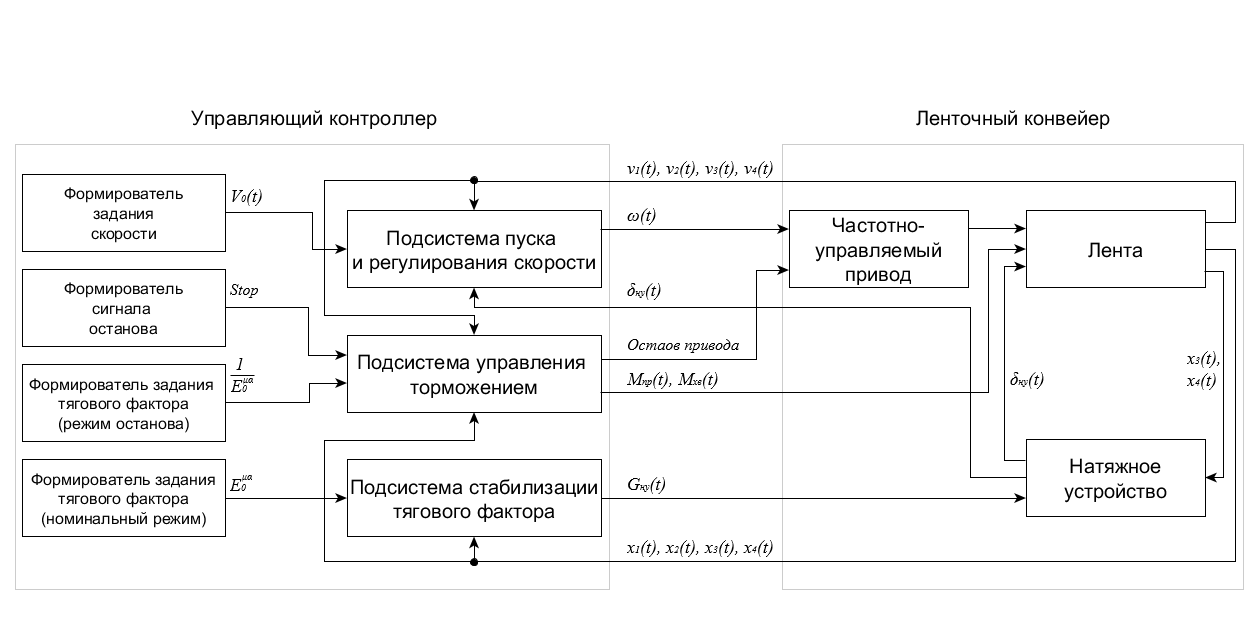
\includegraphics [scale=0.75] {commonSheme.png}
  \caption{Общая структурная схема комплексной автоматической системы управления конвейерной установкой} 
  \label{img.5.common}  
\end{figure}
\end{landscape}

В схеме приняты следующие обозначения: $ M_{\text{пр}}(t) $ -- движущий момент привода, $ v(t) $  -- текущие скорости движения характерных точек ленты, $ V_0(t) $ -- заданное значение скорости привода, $ \omega(t) $ -- частота вращения ротора привода, $ G_{\text{ну}}(t) $ -- текущее натяжение, создаваемое весом натяжного устройства, $ E^{\mu \alpha}(t) $ -- текущее значение тягового фактора, $ E_0^{\mu \alpha} $ -- заданное значение тягового фактора для номинального режима работы, $ \frac{1}{E_0^{\mu \alpha}} $ -- заданное значение тягового фактора для режима останова, $ \delta_{\text{ну}}(t) $  -- перемещение натяжного устройства, $ M_{\text{Тпр}}(t) $ -- значение тормозного момента, прикладываемого к приводному барабану, $ M_{\text{Тхв}}(t) $ -- значение тормозного момента, прикладываемого к хвостовому барабану.\\

\textbf{Подсистема пуска и регулирования скорости} содержит в себе оптимальный регулятор скорости, разработанный на основе метода А.М. Летова \cite{vdmitrieva}. В качестве критерия оптимальности был выбран функционал, который интегрально характеризует качество переходных процессов и величину энергетических затрат на движение~\cite{AKrasovsky}:

$$ I = 0,5\int_0^T [X^T(t) QX(t) + U^T(t)RU(t)]dt, $$

где $ Q $ и $ R $ -- положительные определенные симметричные матрицы.

Оптимальное управление в этом случае формируется по следующему закону:

$$ U(t) = -KX(t) + K(-(A-BK))^{-1}BU^*(t) + U^*(t), $$
 
где $ K $ -- матрица обратных связей, которая определяется согласно процедуре принципа максимума Л. С. Понтрягина~\cite{EGaleev}. Структурная схема регулятора, соответствующая этому закону управления, представлена на рис.~\ref{img.5.speed_controller}.

\begin{figure} [h] 
  \center
  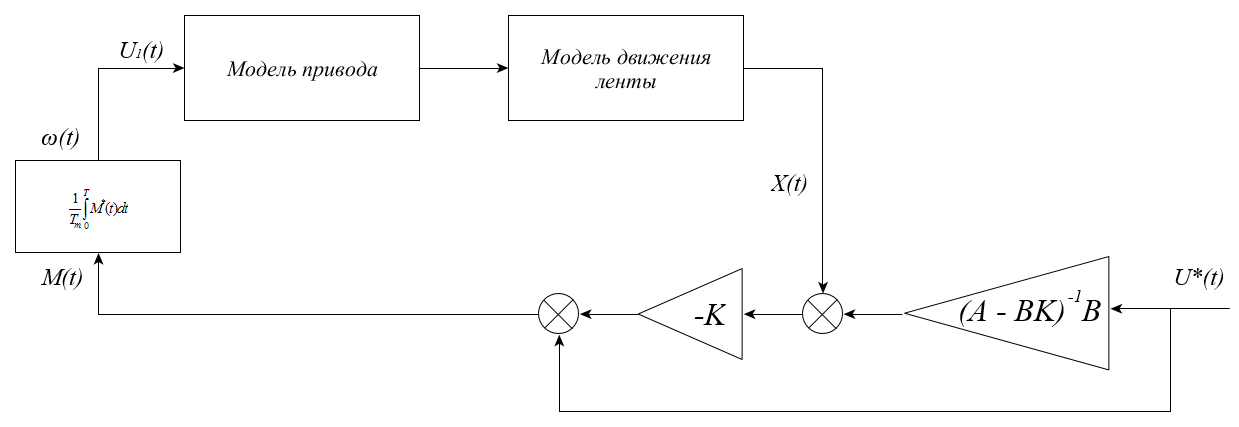
\includegraphics [scale=0.5] {optimal1.png}
  \caption{Структурная схема регулятора скорости} 
  \label{img.5.speed_controller}  
\end{figure}

Подсистема пуска и регулирования скорости работает в двух режимах. В режиме пуска подсистема получает задания скорости $ V_{\text{0 пуск}} $ и $ V_{\text{0 ном}} $ и осуществляет пуск конвейера и вывод на ползучую скорость $ V_{\text{0 пуск}} $, ожидает завершения переходных процессов в ленте и переключает скорость на номинальную $ V_{\text{0 ном}} $. В режиме регулирования скорости подсистема получает задание скорости $ V_0(t) $, которое зависит от внешних условий (например, от случайно изменяющегося грузопотока), получает текущее значение скорости приводного барабана и положения натяжного устройства, и осуществляет переключение скорости движения ленты посредством изменения частоты вращения вращения ротора привода по закону оптимального управления.\\

\textbf{Подсистема стабилизации тягового фактора} содержит в себе блок расчета текущего значения тягового фактора, реализованный согласно структурной схеме, изображенной рна рис.~\ref{img:3.ema1}, и регулятор, осуществляющий управление усилиями в канатах натяжного устройства в зависимости от текущей величины тягового фактора при работе конвейера в номинальном режиме. Стабилизация тягового фактора осуществляется для исключения проскальзывания ленты на приводном барабане при переключении скорости ее движения в номинальном режиме работы конвейера и достигается за счет изменения значений натяжений в характерных точках ленты. Регулятор натяжения подробно описан в работе \cite{vdmitrieva}.

Подсистема стабилизации тягового фактора получает задание тягового фактора для номинального режима работы $ E_0^{\mu \alpha} $, рассчитанное на основе параметров используемого конвейера, и текущие значения перемещений в характерных точках ленты. На основе текущих значений перемещений подсистема вычисляет текущие значения натяжений в характерных точках ленты и, следовательно, текущую величину тягового фактора (\ref{sect3_4}). Регулятор натяжения формирует сигнал управления на основе текущего значения тягового фактора и значения задания по определенному закону. Структурная схема подсистемы стабилизации тягового фактора представлена на рис.~\ref{img.5.pullfactor}.\\

\begin{figure} [h] 
  \center
  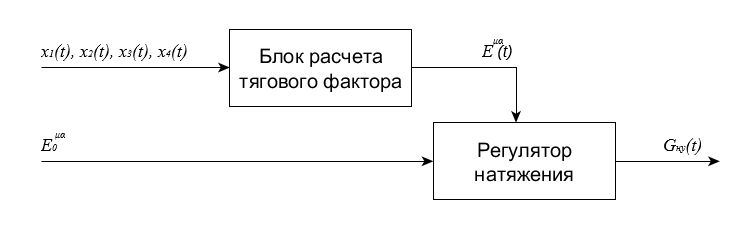
\includegraphics [scale=0.55] {5-2.png}
  \caption{Структурная схема подсистемы стабилизации тягового фактора} 
  \label{img.5.pullfactor}  
\end{figure}

\textbf{Подсистема управления торможением} содержит в себе блок расчета текущего значения тягового фактора для режима торможения, реализованный согласно структурной схеме, изображенной рна рис.~\ref{img:3.ema1}, и блок формирования управляющих сигналов для останова привода и для управления тормозными устройствами. Подсистема является реализацией алгоритма предварительного управляемого торможения конвейера, описанного в главе \ref{chapt4}. Структурная схема подсистемы управления торможением представлена на рис.~\ref{img.5.brake}.

\begin{figure} [h] 
  \center
  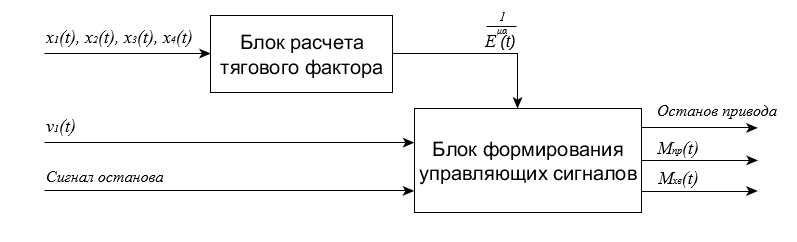
\includegraphics [scale=0.55] {5-3.png}
  \caption{Структурная схема подсистемы управления торможением} 
  \label{img.5.brake}  
\end{figure}

Описанная структура комплексной системы управления конвейерной установкой позволяет наглядно видеть взаимосвязи между управляющими компонентами системы и компонентами объекта управления, а также внутреннюю структуру управляющих компонентов, определить параметры и сигналы объекта управления, необходимые для работы управляющих компонентов.

Техническая реализация системы управления согласно описанной структуре позволит реализовать каждую управляющую подсистему в виде независимого функционального блока (блоков), что согласовывается с современными стандартами разработки систем управления на основе решений ведущих производителей специализированного программного и аппаратного обеспечения. Это также облегчит разработку и отладку системы, сделает возможным использовать компоненты системы независимо друг от друга, расширять функциональность системы, добавляя новые требуемые алгоритмы управления и без какого-либо ущерба использовать известные средства резервирования и повышения отказоустойчивости, применяемые  в промышленных системах автоматизации и управления.\\

Согласно общей структурной схеме системы управления, оборудование, составляющее аппаратную платформу системы, должно принимать один дискретный сигнал, инициирующий останов конвейера и шесть аналоговых сигналов (входные аналоговые каналы) для получения следующей информации:
\begin{itemize}
\item скорость первой сосредоточенной массы $ v_1(t) $;
\item скорость второй сосредоточенной массы $ v_2(t) $;
\item скорость третьей сосредоточенной массы $ v_3(t) $;
\item скорость четвертой сосредоточенной массы $ v_4(t) $;
\item положение натяжного устройства $ \delta_\text{ну}(t) $;
\item задание скорости движения ленты.
\end{itemize}

Также оборудование должно иметь один дискретный выходной канал для управления пуском и остановом привода и четыре аналоговых выходных канала для формирования управляющих воздействий:
\begin{itemize}
\item частота вращения ротора привода $ \omega(t) $;
\item усилие в канатах натяжного устройства $ G_{\text{ну}}(t) $;
\item тормозной момент приводного барабана $ M_\text{Т пр}(t) $;
\item тормозной момент хвостового барабана $ M_\text{Т хв}(t) $.
\end{itemize}

Комплексная система автоматического управления ленточного конвейера является распределенной системой, что обусловлено значительной длиной конвейерной установки. Это предполагает использование нескольких коммуникационных модулей (устройств связи с объектом, УСО) и одного управляющего программируемого контроллера, объединенных между собой посредством промышленной сети передачи данных. Коммуникационные модули получают данные с первичных преобразователей, осуществляют их нормализацию и конвертацию в цифровой вид, обеспечивают гальваническую развязку с сетью передачи данных. Также коммуникационные модули преобразовывают управляющие сигналы, формируемые контроллером, в сигналы для исполнительных механизмов. Управляющий контроллер осуществляет сбор данных от коммуникационных модулей, обеспечивает работу управляющих алгоритмов и передает формируемые ими управляющие сигналы на коммуникационные модули.

В качестве сети передачи данных предлагается использовать промышленную сеть стандарта Profibus. Profibus -- это открытый международный стандарт, который описывает шинную систему, предназначенную для установления связи с процессами и полевыми устройствами на полевом уровне, а также для обмена данными в пределах отдельной ячейки автоматизации. Физически Profibus может представлять собой электрическую сеть с шинной топологией, использующую экранированную витую пару, соответствующую стандарту RS-485, оптическую сеть на основе волоконно-оптического кабеля или инфракрасную сеть. Скорость передачи по ней может варьироваться от 9,6 Кбит/сек до 12 Мбит/сек.\\

Особенностью ленточного конвейера с натяжным устройством, расположенным в хвостовой части, как объекта автоматизации является подвижный хвостовой барабан. Хвостовой барабан жестко соединен с автоматическим натяжным устройством посредством канатов. Натяжное устройство в процессе работы конвейера изменяет усилия с канатах для управления натяжениями в ленте. Из-за этого хвостовой барабан, на котором расположено тормозное устройство, осуществляет перемещения. Для управления тормозным устройством хвостового барабана необходимо соединение его исполнительного механизма с коммуникационным модулем вывода. Согласно результатом модельных исследований (рис.~\ref{img:3.pdx}), натяжное устройство перемещает хвостовой барабан конвейера в пределах 15 метров, что делает невозможным использование прямого проводного соединения исполнительного механизма тормозного устройства с коммуникационным модулем.

Для решения этой проблемы автор предлагает использовать беспроводную промышленную коммуникационную сеть. Для этого необходима установка отдельного коммуникационного модуля вместе с тормозным устройством на тележке хвостового барабана. Этот коммуникационный модуль соединяется с принимающим устройством (антенной), также расположенной на тележке хвостового барабана, которая осуществляет прием управляющих сигналов от неподвижного передающего устройства (точки доступа), подключенного к общей сетевой инфраструктуре системы автоматического управления.

В качестве беспроводной сети передачи данных предлагается использование сети стандарта IEEE 802.11. Характеристики такой сети приведены в таблице~\ref{tabl.5:802.11b}. 

\begin{table}[h!]
\caption{Характеристики беспроводной сети передачи данных на основе стандарта IEEE 802.11b}
\label{tabl.5:802.11b}

\begin{center}
\begin{tabular}{|p{0.4\linewidth}|p{0.5\linewidth}|}
\hline
Характеристика                    & Значение     \\
\hline
Полоса частот                     & 2,4 ГГц      \\
\hline
Скорость передачи данных          & 11 Мбит/сек  \\
\hline
Непересекающиеся каналы           & 3            \\
\hline
Мощность передачи                 & 100 мВт      \\
\hline
Модуляция                         & DSSS         \\
\hline
Проникновение через стены         & Среднее      \\
\hline
Отражения                         & Сильные      \\
\hline
Опасность помех от радиоустройств & Средняя      \\
\hline
 
\end{tabular}
\end{center}
\end{table}

Применение беспроводных технологий в системах автоматизации накладывает определенные требования к стандарту передачи данных. Промышленная реализация беспроводных сетей обеспечивает возможность расширения требований стандарта IEEE 802.11 на системы промышленной связи. При этом обеспечивается детерминированное время обмена данными, возможность использования резервированных беспроводных каналов связи, возможность использования одной сети для передачи как критичных (например, аварийных), так и не критичных (например, сервисных или диагностических) сообщений. Особенности промышленных беспроводных сетей описаны в~\cite{siemens5}.

\begin{landscape}
\begin{figure} [h] 
  \center
  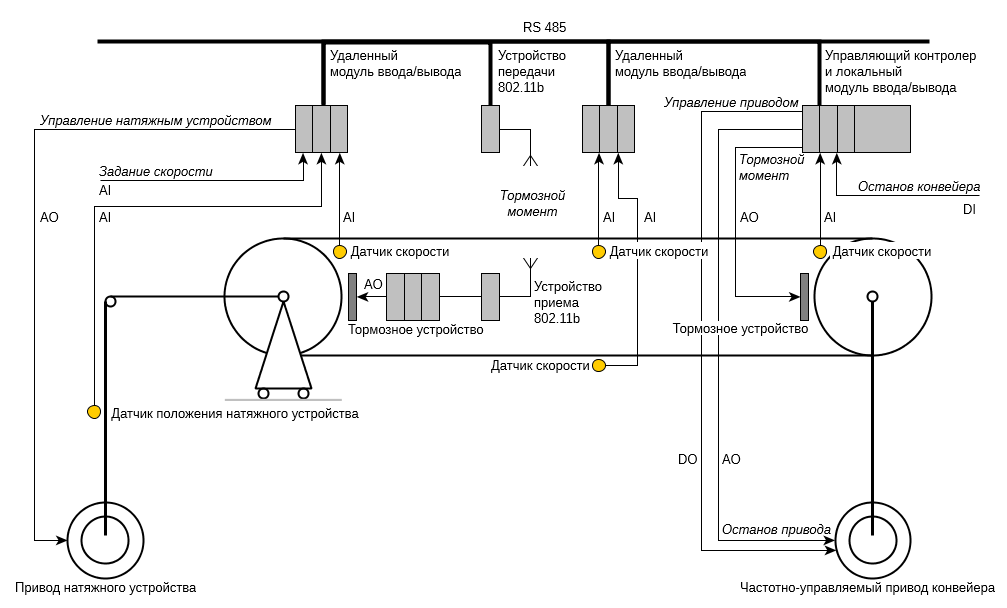
\includegraphics [scale=1] {5-4.png}
  \caption{Общая схема технической реализации комплексной системы управления конвейерной установкой} 
  \label{img.5.TechR}  
\end{figure}
\end{landscape}

\section{Выбор управляющего программного и аппаратного обеспечения для технической реализации комплексной автоматизированной системы управления конвейерной установкой} \label{sect5_2}

Для технической реализации комплексной системы управления конвейерной установкой требуется следующий комплекс программного и аппаратного обеспечения:
\begin{itemize}
\item программируемые логические контроллеры для вычисления управляющих сигналов в соответствии с реализованными алгоритмами управления;
\item устройства связи с объектом (УСО, коммуникационные модули) для преобразования сигналов от измерительных устройств к виду, пригодному для использования при расчетах, а также для преобразования управляющих сигналов, формируемых программируемым контроллером к виду, адаптированному для того или иного исполнительного устройства;
\item источники питания для оборудования системы управления;
\item измерительные устройства (датчики) для измерения требуемых параметров объекта управления;
\item специализированное ПО (среда разработки и компиляторы) для программирования алгоритмов управления с возможностью выполнения их на программируемом контроллере;
\item система верхнего уровня для диспетчерского управления и сбора данных (SCADA).
\end{itemize}

Основой разрабатываемой системы управления является техническая реализация разработанных ранее алгоритмов управления на современном промышленном аппаратном обеспечении (программируемых логических контроллерах), поэтому технологии создания программного обеспечения для систем, построенных на базе ПЛК, следует уделить особое внимание. Реализованные алгоритмы должны соответствовать современным стандартам промышленного программного обеспечения и иметь возможность выполняться на различном оборудовании (быть легко переносимыми). Поэтому при реализации алгоритмов управления целесообразно следовать стандарту МЭК 61131-3, описывающему промышленные языки программирования для программируемых логических контроллеров~\cite{ipetrov}.\\

\subsection{Выбор программируемого контроллера и среды разработки алгоритмов} \label{subsect5_2_1}

На рынке средств промышленной автоматизации в настоящее время представлены разнообразные аппаратные и программные средства разработки систем управления. При выборе комплекса оборудования и программного обеспечения для построения системы управления необходимо учитывать совместимость компонентов системы между собой (контроллеры, коммуникационные модули, источники питания и т. д.), а также поддержку выбранным оборудованием средств и языков программирования стандарта МЭК 61131-3.

Задачу выбора аппаратного и программного обеспечения для разрабатываемой системы можно решить путем использования комплексных решений от ведущих мировых производителей, предлагающих функционально полный набор ПЛК, коммуникационных модулей ввода/вывода, дополнительного оборудования и совместимое с ними программное обеспечение.

В качестве аппаратной платформы выберем программируемый контроллер SIMATIC S7-300 с центральным процессором CPU 312, который производится концерном Siemens, а в качестве программного обеспечения для реализации алгоритмов управления выберем среду Simatic Step 7, которая представляет собой специализированное программное обеспечение для создания и обслуживания систем автоматизации на основе программируемых логических контроллеров Simatic S7-300 и Simatic S7-400 фирмы Siemens.

Преимущество выбранной платформы состоит в том, что производитель выпускает все необходимые компоненты, включая источники питания и модули связи с объектами и обеспечивает их полноценную совместимость между собой.\\

Программируемые контроллеры SIMATIC S7-300 допускают  использование  в  жестких  внешних условиях.  Они  имеют  расширенный  температурный  рабочий  диапазон: $ (-25...+60)^\circ С, $ повышенную  вибрационную  и  ударную  стойкость, соответствующие стандарту IEC 68 часть 2-6, удовлетворяют требованиям по влагостойкости, устойчивости к образованию конденсата и инея согласно IEC 721-3-3 Class 3 K5~\cite{siemens2}.

Программируемый контроллер SIMATIC S7-300/400 имеет модульную конструкцию. Модули, из которых составляется требуемая конфигурация контроллера, могут быть центральными (располагаться по соседству с центральным процессором) или распределенными. В системах SIMATIC S7 распределенные  входы/выходы являются составной частью системы. Центральный процессор, имеющий различные области памяти, составляет основу оборудования системы для обработки программ пользователя. Загрузочная память (load memory) целиком содержит пользовательскую программу; части программы, выполняемые в любое заданное время (исполняемый модуль программы), находятся в рабочей памяти (work memory), обеспечивающей малое время доступа к данным, что обеспечивает высокую скорость обработки данных~\cite{siemens2}. Общий вид программируемого контроллера SIMATIC S7-300 представлен на рис.~\ref{img.5.cpu312}.

\begin{figure} [h!] 
  \center
  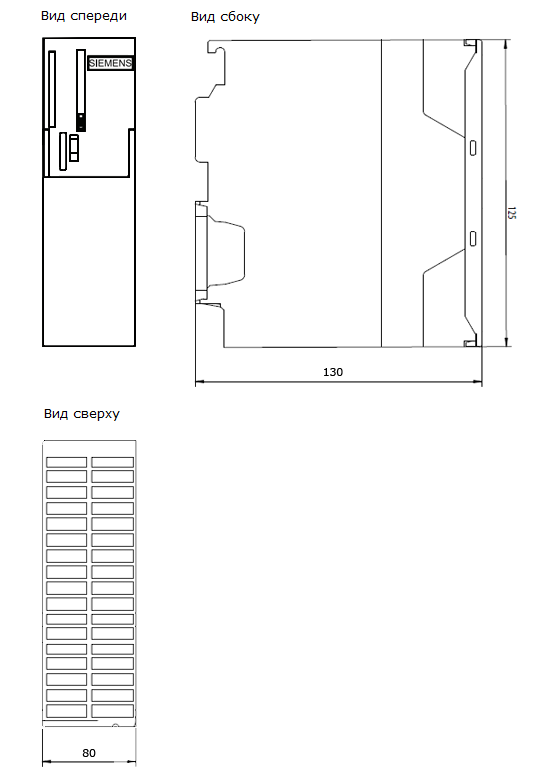
\includegraphics [scale=0.55] {cpu312.png}
  \caption{Общий вид программируемого контроллера SIMATIC S7-300} 
  \label{img.5.cpu312}  
\end{figure}

Технические характеристики выбранного оборудования представлены в табл.~\ref{5.tabl:S7-300}.\\

\begin{table}[h!]
\caption{Технические характеристики программируемого контроллера SIMATIC S7-300 с центральным процессором CPU 312}
\label{5.tabl:S7-300}

\begin{center}
\begin{tabular}{|p{0.4\linewidth}|p{0.5\linewidth}|}
\hline
Характеристика                                   & Значение                                 \\
\hline
Степень защиты корпуса                           & IP 20 в соответствии с IEC 60 529        \\
\hline
Рабочие температуры при горизонтальной установке & $ (-25...+60)^\circ С $                  \\
\hline
Рабочие температуры при вертикальной установке   & $ (-25...+40)^\circ С $                  \\
\hline
Относительная влажность                          & 5 ... 95\%                               \\
\hline
Атмосферное давление                             & 795 ... 1080 ГПа                         \\
\hline    
Встроенная память                 & 32 Кбайт                                                \\
\hline    
Цифровые каналы                   &                                                         \\
\hline    
-- встроенные каналы (DI)         & 10                                                      \\
\hline    
-- встроенные каналы (DO)         & 6                                                       \\
\hline    
-- входы                          & 266                                                     \\
\hline    
-- выходы                         & 262                                                     \\
\hline    
-- входы, центральные             & 266                                                     \\
\hline    
-- выходы, центральные            & 262                                                     \\
\hline    
Аналоговые каналы                 &                                                         \\
\hline    
-- встроенные каналы (AI)         & нет                                                     \\
\hline    
-- встроенные каналы (AO)         & нет                                                     \\
\hline    
-- входы                          & 64                                                      \\
\hline    
-- выходы                         & 64                                                      \\
\hline    
-- входы, центральные             & 64                                                      \\
\hline    
-- выходы, центральные            & 64                                                      \\
\hline
Импульсные выходы                 & 2 канала с широтно-импульсной модуляцией, макс. 2,5 кГц \\
\hline    
Интерфейсы                        &                                                         \\
\hline    
Тип интерфейса                    & RS 485                                                  \\
\hline    
Потенциальная развязка            & Нет                                                     \\
\hline    
Электропитание на интерфейсе      & макс. 200 мА                                            \\
\hline    
Программирование                  &                                                         \\
\hline    
Языки программирования            & LAD/FBD/STL/SCL                                         \\
\hline    
Защита программы пользователя     & Да                                                      \\
\hline    
Монтажные размеры Ш х В х Г (мм)  & 80 x 125 x 130                                          \\
\hline    
Масса                             & 409 г                                                   \\
\hline    
Питающее напряжение               & 24 В пост. тока                                         \\
\hline
Потребление тока 
(номинальная величина)            & 500 мА                                                  \\
\hline
Мощность потерь                   & 6 Вт                                                    \\
\hline

\end{tabular}
\end{center}
\end{table} 

\subsection{Выбор коммуникационных модулей} \label{subsect5_2_2}

Согласно рис.~\ref{img.5.TechR}, для построения распределенной системы управления требуется три группы коммуникационных модулей ввода/вывода. 

Первая группа модулей принимает аналоговый сигнал датчика скорости участка грузовой ветви ленты у приводного барабана, осуществляет вывод аналоговых и дискретных сигналов управления приводом и тормозным устройством приводного барабана.

Вторая группа модулей принимает аналоговые сигналы датчиков скорости участка ленты центра грузовой ветви и участка ленты центра порожней ветви, которые расположены относительно близко друг к другу.

Третья группа модулей принимает аналоговые сигналы датчика скорости участка ленты грузовой ветви у хвостового барабана и датчика положения натяжного устройства, а также осуществляет вывод аналоговых сигналов управления натяжным устройством и тормозным устройством хвостового барабана.

Для ввода/вывода аналоговых сигналов выберем коммуникационные модули SM 334; AI 4/AO 2 x 12 Bit производства Siemens~\cite{siemens3}. Эти модули имеют 4 аналоговых входа в 2 группах и 2 аналоговых выхода в одной группе с разрешающей способностью 12 битов + знак на канал. Модули имеют гальваническую развязку с интерфейсом задней шины и с напряжением на нагрузке и поддерживают измерение напряжения, сопротивления или температуры. Общий вид коммуникационного модуля представлен на рис.~\ref{img.5.SM334}.

\begin{figure} [h!] 
  \center
  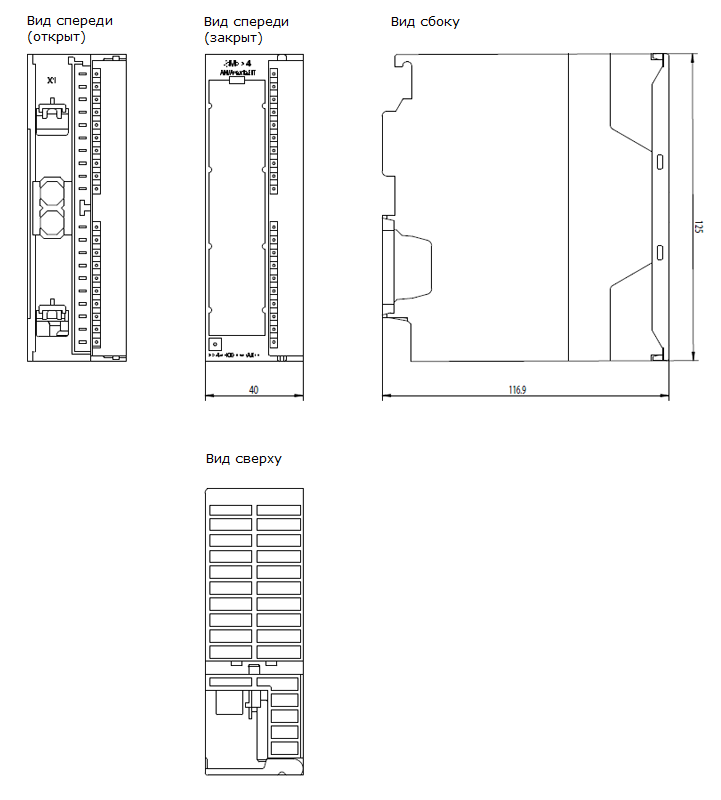
\includegraphics [scale=0.5] {sm334.png}
  \caption{Общий вид аналогового коммуникационного модуля SM 334; AI 4/AO 2 x 12 Bit} 
  \label{img.5.SM334}  
\end{figure}

Технические характеристики выбранного аналогового коммуникационного модуля представлены в табл.~\ref{5.tabl:SM334}.\\

Для ввода/вывода дискретных сигналов выберем коммуникационные модули SM 323; DI 8/DO 8 производства Siemens~\cite{siemens3}. Эти модули имеют 8 дискретных входов и 8 дискретных выходов. Модули имеют гальваническую развязку и пригодны для получения дискретных сигналов от переключателей и для вывода дискретных сигналов для электромагнитных вентилей, контакторов постоянного тока и индикаторных ламп.
Общий вид коммуникационного модуля представлен на рис.~\ref{img.5.SM323}.

\begin{figure} [h!] 
  \center
  \includegraphics [scale=0.4] {sm323.png}
  \caption{Общий вид дискретного коммуникационного модуля SM 323; DI 8/DO 8} 
  \label{img.5.SM323}  
\end{figure}

Технические характеристики выбранного аналогового коммуникационного модуля представлены в табл.~\ref{5.tabl:tSM323}.\\
 
\begin{table}[h!]
\caption{Технические характеристики коммуникационного модуля SM 334 AI 4/AO 2x12 Bit}
\label{5.tabl:SM334}
 
\begin{center}
\begin{tabular}{|p{0.4\linewidth}|p{0.5\linewidth}|}
\hline
Характеристика                           & Значение              \\
\hline
Размеры, Ш х В х Г (мм)                  & 40 х 125 х 117        \\
\hline
Вес (гр)                                 & 200                   \\
\hline
Число входов                             & 4                     \\
\hline
Число выходов                            & 2                     \\
\hline
Длина кабеля                             & макс. 100 м           \\
\hline
Номинальное напряжение источника питания & 24 В постоянного тока \\
\hline
Принцип измерения                        & Интегрирующий         \\
\hline
Входные диапазоны, напряжение            & от 0 до 10 В          \\
\hline
Входные диапазоны, сопротивление         & 10 кОм                \\
\hline
Входные диапазоны, сопротивление         & 10 кОм                \\
\hline
Входные диапазоны, температура           & Pt 100                \\
\hline
Выходной диапазон, напряжение            & от 0 до 10 В          \\
\hline
 
\end{tabular}
\end{center}
\end{table} 

\begin{table}[h!]
\caption{Технические характеристики коммуникационного модуля SM 323; DI 8/DO 8}
\label{5.tabl:tSM323}
 
\begin{center}
\begin{tabular}{|p{0.4\linewidth}|p{0.5\linewidth}|}
\hline
Характеристика                               & Значение              \\
\hline
Размеры, Ш х В х Г (мм)                      & 40 х 125 х 117        \\
\hline 
Вес (гр)                                     & 200                   \\
\hline
Число входов                                 & 8                     \\
\hline
Число выходов                                & 8                     \\
\hline
Длина кабеля                                 & макс. 1000 м          \\
\hline
Напряжение питания                           & 24 В постоянного тока \\
\hline
Потенциальная развязка                       & Да                    \\
\hline
Данные для выбора датчика                    &                       \\
\hline
номинальное значение входного напряжения     & 24 В пост. тока       \\
\hline
значение напряжения для сигнала <<1>>        & от 13 до 24 В         \\ 
\hline
значение напряжения для сигнала <<0>>        & от – 30 до 5 В        \\
\hline
Входной ток                                  & тип. 7 мА             \\
\hline
Входная характеристика                       & в соответствии с МЭК 61131 -- 1 \\
\hline
Данные для выбора исполнительного устройства &                       \\
\hline
Выходное напряжение                          & мин. L + (- 0,8 В)    \\
\hline
Выходной ток                                 & 0,5 мА                \\
\hline
Диапазон сопротивления нагрузки              & от 48 Ом до 4 кОм     \\
\hline
 
\end{tabular}
\end{center}
\end{table}

\subsection{Выбор источников питания} \label{subsect5_2_3}

Все выбранные аппаратные компоненты системы управления требуют питания 24 В постоянного тока. В качестве источника питания выберем Блок питания PS~307;~2~A~\cite{siemens3}. Отличительной особенностью этого блока питания является то, что он может использоваться не только для питания электроники коммуникационных модулей и программируемого контроллера, но и для питания цепей датчиков и исполнительных устройств. Технические характеристики выбранного источника питания представлены в табл.~\ref{5.tabl:PS307}

\begin{table}[h!]
\caption{Технические характеристики бока питания PS~307;~2~A}
\label{5.tabl:PS307}
 
\begin{center}
\begin{tabular}{|p{0.4\linewidth}|p{0.5\linewidth}|}
\hline
Характеристика          & Значение                            \\
\hline
Размеры, Ш х В х Г (мм) & 40 х 125 х 117                      \\
\hline
Вес (гр)                & 420                                 \\
\hline
Входное напряжение      & 120 / 230 В переменного тока        \\
\hline
Частота сети            & 50 -- 60 ГЦ                         \\
\hline
Номинальный входной ток & 0,5 А                               \\
\hline
Выходное напряжение     & 24 В постоянного тока ($ \pm 5 \%$) \\
\hline
Выходной ток            & 2 А                                 \\
\hline
Остаточные пульсации    & макс. 150 мВ (пиковое значение)     \\
\hline
К.П.Д.                  & 83\%                                \\
\hline
Потребляемая мощность   & 58 Вт                               \\
\hline
 
\end{tabular}
\end{center}
\end{table}      

\subsection{Выбор первичных преобразователей (датчиков)} \label{subsect5_2_4}

Система управления получает от объекта только информацию о скоростях перемещения характерных точек конвейерной ленты и натяжного устройства. Это аналоговые сигналы, значения которых используются как входные параметры управляющих алгоритмов. Для получения этих сигналов необходимо измерять линейную скорость движения ленты и перемещения натяжного устройства. Для этих целей можно использовать тахометрические датчики скорости, например М4207 или ИДС-2. Это измерительные устройства, разработанные специально для применения на конвейерном транспорте для измерения скорости движения ленты. Принцип работы этих датчиков основан на преобразовании поступательного движения конвейерной ленты во вращательное движение вала датчика скорости и генерации электрических импульсов, частота которых пропорциональна скорости вращения вала. Измерительное колесо с помощью конструктивных элементов прижимается к движущейся ленте и преобразует поступательное движение ленты во вращательное движение вала. На валу в корпусе установлен оптический датчик вращения, который имеет разрешение 1000 импульсов на один оборот измерительного колеса. Электрические импульсы могут передаваться по кабелю связи в обрабатывающее устройство (коммуникационный модуль) для вычисления скорости перемещения ленты конвейера.

Плата электрического преобразователя расположена в корпусе за оптическим датчиком. Плата содержит клеммные соединители для подключения информационных и питающих цепей датчика, схему дешифратора сигналов с датчика, схему питания и клеммный соединитель для подключения кабеля связи. Выходной каскад схемы -- открытый коллектор. Это позволяет повысить помехоустойчивость линии связи с коммуникационным модулем. Кабель связи пропускается в корпус датчика через герметичный кабельный ввод.

Датчик скорости предназначен для работы в помещениях и на открытом воздухе при температуре окружающего воздуха от минус 30 до плюс $40^\circ$ C, при относительной влажности не более 80 \% при температуре $25^\circ$ C, атмосферном давлении от 84 до 106,7 кПа (от 630 до 800 мм рт. ст.). Вид климатического исполнения УХЛ 2 по ГОСТ 15150--69.

\subsection{Выбор языка программирования для реализации алгоритмов управления} \label{subsect5_2_5}

Для реализации алгоритмов управления выберем язык SCL~\cite{siemens4}, который является специализированным языком высокого уровня для программирования промышленных контроллеров. Синтаксис языка SCL подобен синтаксису языка Pascal. SCL позволяет программировать сложные алгоритмы, математические функции, решать задачи управления данными и оптимизации вычислений. Реализация языка SCL, включенная в среду разработки SIMATIC S7, согласуется с концепцией функциональных блоков. Текст программы требует компиляции, результатом которой является функциональный блок, реализующий запрограммированный алгоритм. Этот блок сохраняется в библиотеке и его можно использовать в других программах (в том числе, написанных на других языках), вызывать его из других функциональных блоков. Кроме того, SCL имеет функции отладки, которые позволяют осуществлять наблюдение за выполнением программы в реальном времени, выполнять программу пошагово на основе указываемых точек останова и пользоваться другими преимуществами средств отладки языков высокого уровня.

\section{Программирование алгоритмов управления} \label{sect5_3}

Настоящий раздел содержит описание реализации алгоритмов управления магистральным ленточным конвейером на промышленном языке программирования SCL, а также общее описание программного обеспечения комплексной системы управления магистральным ленточным конвейером, структура которой описана в \ref{sect5_1}.

\subsection{Об особенностях разработки программного обеспечения для ПЛК Simatic S7--300} \label{subsect5_3_1}
Программа контроллера Simatic S7--300 выполняется циклически с жестко заданным временем цикла. При включении контроллера однократно выполняется последовательность вычислений, заданная в блоке запуска (OB100), после этого запускается мониторинг времени цикла и в качестве первой операции цикла осуществляется считывание состояний сигналов из модулей и сохранение данных в области отображения процесса. Далее осуществляется выполнение основной программы, которая должна содержаться в определенном блоке OB1 (cycle execution), при этом может осуществляться обработка прерываний от аппаратных устройств или вызов других функциональных блоков или функций. В конце цикла происходит запись результатов работы программы в область памяти модулей вывода.

Программа состоит из набора функциональных блоков, каждый из которых имеет входы и выходы и выполняет определенную операцию. На входы функциональных блоков могут поступать входные значения параметров из области памяти коммуникационных модулей ввода, либо значения с выходов других функциональных блоков. Параметры с выходов могут поступать в соответствующие области памяти коммуникационных модулей вывода, либо на входы других функциональных блоков. Пользователь имеет возможность разрабатывать собственные функциональные блоки, либо использовать готовые функциональные блоки системной библиотеки.

Настоящая реализация алгоритмов комплексной автоматизированной системы управления ленточным конвейером предполагает разработку отдельных функциональных блоков для каждого алгоритма или вычислительной операции с последующим объединением их в общую управляющую программу.

\subsection{Функциональный блок расчета параметров управляющих алгоритмов} \label{subsect5_3_2}
Блок расчета параметров управляющих алгоритмов реализуется в соответствии с разработанной методикой расчета (\ref{sect4_5}) и осуществляет расчет требуемых параметров и уставок управляющих алгоритмов. Для разных типов конвейеров эти параметры могут отличаться, поэтому блок предусматривает набор констант, которые задаются в соответствии с типом используемого конвейера. Данный блок целесообразно размещать в организационном блоке OB100 для того, чтобы расчет параметров и уставок осуществлялся однократно при включении управляющего контроллера.

Исходный код программы расчета параметров управляющих алгоритмов представлен в приложении~\ref{AppendixB1}. Функциональный блок не имеет входов и рассчитывает следующие параметры: задающие значения тягового фактора для номинального режима работы конвейера и для режима торможения, значения тормозных моментов для приводного и хвостового барабанов.

Графическое представление разработанного функционального блока в среде разработки Step 7 представлено на рис.~\ref{img.5.fb_init}.

\begin{figure} [h!] 
  \center
  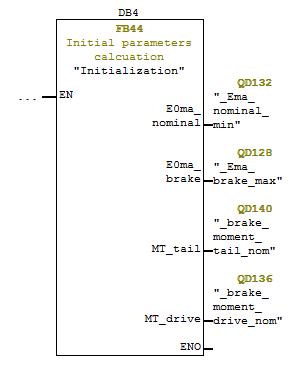
\includegraphics [scale=0.75] {5-3-2-0.png}
  \caption{Графическое представление функционального блока расчета параметров управляющих алгоритмов}
  \label{img.5.fb_init}  
\end{figure}

\subsection{Функциональный блок расчета текущего значения тягового фактора} \label{subsect5_3_3}
Расчет текущего значения тягового фактора используется в двух алгоритмах (\ref{sect5_1}) -- алгоритме стабилизации тягового фактора в номинальном режиме работы конвейера и алгоритме управляемого торможения конвейера, поэтому целесообразно описать его реализацию отдельно. Реализация расчета текущего значения тягового фактора в Simulink приведена в разделе \ref{sect3_4}, структурная схема представлена на рис. \ref{img:3.ema1}. В соответствии с ней реализован функциональный блок, получающий на входы аналоговые сигналы, соответствующие текущим величинам перемещений характерных точек конвейерной ленты. Выходы блока формирують аналоговые величины, соответствующие текущему значению тягового фактора и натяжениям в точках набегания ленты на приводной барабана и сбегания ленты с приводного барабана.

Текущие значения перемещений характерных точек ленты вычисляются путем интегрирования получаемых величин скоростей этих кочек от коммуникационных модулей. Интегрирование осуществляется посредством специального функционального блока, реализующего алгоритм численного расчета интеграла входной величины. Этот алгоритм также реализован на языке SCL выполняется в блоке OB35, который реализует циклические прерывания центрального процессора каждые 100 мс. Исходный код алгоритма представлен в приложении~\ref{AppendixB5}. 

Исходный код программы вычисления текущего значения тягового фактора представлен в приложении~\ref{AppendixB2}. Функциональный блок имеет четыре аналоговых входа, предназначенных для получения текущих значений перемещений характерных точек ленты, и четыре аналоговых выхода, формирующих текущие значения тягового тягового фактора для номинального режима работы конвейера и для режима торможения, а также текущие величины натяжений в ветвях конвейера. В коде предусмотрен набор констант, соответствующих коэффициентам зависимостей натяжений от деформаций ленты (\ref{eq:s1}, \ref{eq:s4}), так как на эти зависимости влияют свойства используемой ленты.

Графическое представление разработанного функционального блока в среде разработки Step 7 представлено на рис.~\ref{img.5.fb_pull_factor}.

\begin{figure} [h!] 
  \center
  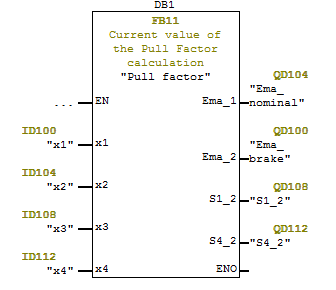
\includegraphics [scale=0.75] {5-3-2-1.png}
  \caption{Графическое представление функционального блока вычисления текущего значения тягового фактора}
  \label{img.5.fb_pull_factor}  
\end{figure}

\subsection{Функциональный блок реализации алгоритма предварительного торможения конвейера} \label{subsect5_3_4}
Данный блок реализует непосредственно алгоритм предварительного торможения конвейера (\ref{sect4_3}) и предназначен для формирования управляющих сигналов для тормозных устройств и устройства управления приводом конвейера. В качестве входных сигналов функциональный блок получает скорости характерных точек ленты, текущее значение тягового фактора для режима торможения, определяемое в блоке расчета текущего значения тягового фактора (\ref{subsect5_3_3}), а также максимальное значение тягового фактора для режима торможения и номинальные значения тормозных моментов, определяемые в блоке расчета параметров управляющих алгоритмов (\ref{subsect5_3_2}). Выходы блока формируют сигнал останова привода и величины тормозных моментов для тормозных устройств.

Исходный код программы реализации алгоритма предварительного торможения конвейера представлен в приложении~\ref{AppendixB3}.

Графическое представление разработанного функционального блока в среде разработки Step 7 представлено на рис.~\ref{img.5.fb_brake}.

\begin{figure} [h!] 
  \center
  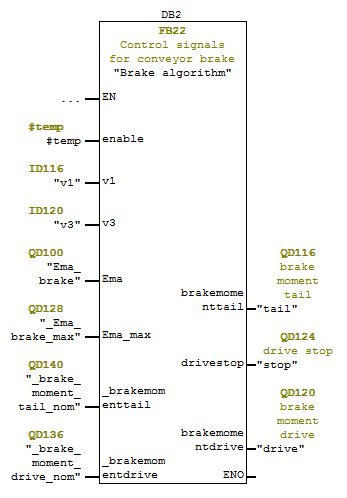
\includegraphics [scale=0.75] {5-3-2-2.png}
  \caption{Графическое представление функционального блока реализации алгоритма предварительного торможения конвейера}
  \label{img.5.fb_brake}  
\end{figure}

\subsection{Функциональный блок реализации регулятора натяжения ленты конвейера} \label{subsect5_3_5}

Данный функциональный блок реализует алгоритм стабилизации тягового фактора в номинальном режиме работы конвейера и формирует управляющие сигналы для изменения положения каретки натяжного устройства. Принцип стабилизации тягового фактора в номинальном режиме работы конвейера основан на полученной в \cite{vdmitrieva} зависимости требуемого веса натяжного устройства от текущего значения тягового фактора.

Исходный код программы реализации алгоритма предварительного торможения конвейера представлен в приложении~\ref{AppendixB4}. Функциональный блок получает на входы текущее значение тягового фактора для номинального режима работы, определяемое в блоке расчета текущего значения тягового фактора \ref{subsect5_3_3}, а также минимальное значение тягового фактора для номинального режима, определяемое в блоке расчета параметров управляющих алгоритмов (\ref{subsect5_3_2}). Выход блока формирует сигнал управления натяжным устройством.  В коде предусмотрен набор констант, соответствующих коэффициентам зависимости требуемого веса натяжного устройства от текущего значения тягового фактора \cite{vdmitrieva}. Структурная схема алгоритма стабилизации тягового фактора представлена на рис. \ref{img.5.fb_Ema_st}. Графическое представление разработанного функционального блока в среде разработки Step 7 представлено на рис.~\ref{img.5.fb_Ema}.

\begin{figure} [h!] 
  \center
  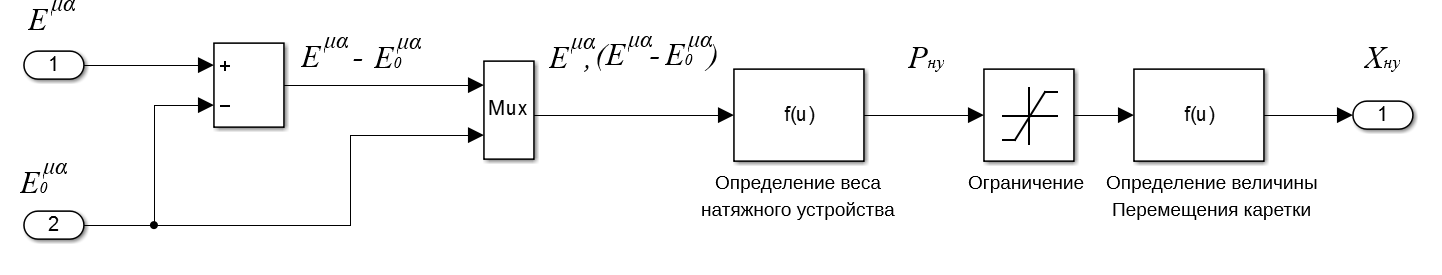
\includegraphics [scale=0.4] {5-3-2-4.png}
  \caption{Структурная схема алгоритма стабилизации тягового фактора}
  \label{img.5.fb_Ema_st}  
\end{figure}

\begin{figure} [h!] 
  \center
  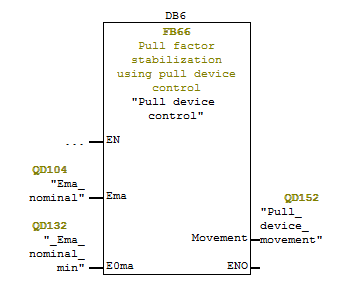
\includegraphics [scale=0.75] {5-3-2-3.png}
  \caption{Графическое представление функционального блока реализации регулятора натяжения ленты конвейера}
  \label{img.5.fb_Ema}  
\end{figure}

\subsection{Функциональный блок реализации оптимального регулятора скорости движения ленты конвейера} \label{subsect5_3_6}

Регулятор скорости вырабатывает сигнал управления в соответствии со следующим законом:

$$ U(t) = -KX(t) + K(-(A-BK))^{-1}BU^*(t) + U^*(t), $$

где $ K_{[3\times10]} $ -- матрица коэффициентов обратных связей по управляющему сигналу, $ X(t)_{[10\times1]} $~-- вектор координат состояния управляемой системы, $ A_{[10\times10]} $ -- матрица состояния управляемой системы, $ B_{[10\times3]} $ -- матрица управления системы, $ U^*(t) $ -- измеряемое управление, пропорционально которому должна быть изменена скорость движения ленты (задание скорости движения ленты).

Как следует из закона управления, для работы оптимального регулятора скорости движения ленты конвейера необходим полный вектор координат состояния управляемой системы. В данном случае это перемещения и скорости характерных точек ленты конвейера и натяжного устройства. Поэтому соответствующий функциональный блок реализации регулятора имеет десять аналоговых входов, принимающих координаты состояния. Значения перемещений характерных точек ленты и натяжного устройства передаются от коммуникационных модулей, значения их скоростей получаются путем дифференцирования перемещений методом определения численного значения производной с использованием разностного отношения. Также функциональный блок принимает задание требуемой скорости движения ленты от формирователя задания скорости, дискретный сигнал пуска конвейера и значение интеграла задания скорости движения ленты.

Регулятор скорости вырабатывает оптимальное управление, пропорциональное движущему моменту привода. Однако управление конвейером должно происходить путем задания частотно-управляемому приводу требуемой частоты вращения. Переход осуществляется путем рования формируемого сигнала управления, поскольку связь между моментом и частотой вращения ротора задается уравнением $T_m \frac{d\omega}{dt} = M $.

Интегрирование задания скорости движения ленты и формируемого оптимального управления осуществляется посредством специального функционального блока, реализующего алгоритм численного расчета интеграла входной величины. Этот алгоритм также реализован на языке SCL выполняется в блоке OB35, который реализует циклические прерывания центрального процессора каждые 100 мс. Исходный код алгоритма представлен в приложении~\ref{AppendixB5}.

Исходный код программы реализации оптимального регулятора скорости движения ленты конвейера представлен в приложении~\ref{AppendixB6}.

Графическое представление разработанного функционального блока в среде разработки Step 7 представлено на рис.~\ref{img.5.fb_drive_control}.

\begin{figure} [h!] 
  \center
  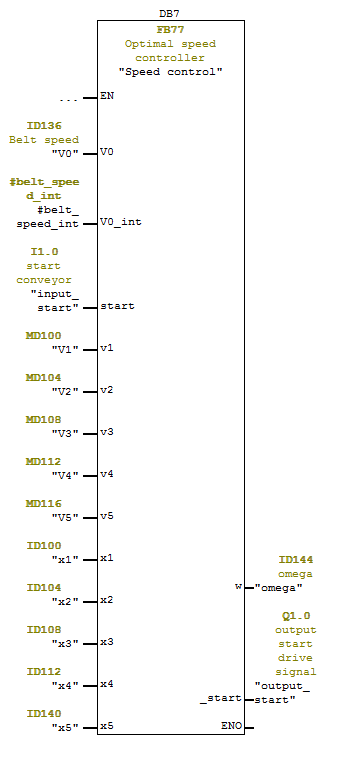
\includegraphics [scale=0.75] {5-3-2-5.png}
  \caption{Графическое представление функционального блока реализации оптимального регулятора скорости движения ленты конвейера}
  \label{img.5.fb_drive_control}  
\end{figure}

\subsection{Основная управляющая программа} \label{subsect5_3_7}

Основная управляющая программа реализует совместное выполнение разработанных алгоритмов управления и представляет собой взаимосвязь описанных выше функциональных блоков. Вызов функциональных блоков, реализующих непосредственно алгоритмы управления, осуществляется циклически с интервалом 100 мс, вызов функциональных блоков, вычисляющих производные и интегралы сигналов, осуществляется циклически по прерываниям, вызов функционального блока, вычисляющего параметры алгоритмов управления, осуществляется при старте и перезапуске контроллера. Исходный код основной программы (на языке ST) представлен в приложении~\ref{AppendixB8}. Список входных, выходных и локальных переменных, которые использует управляющая программа, представлен в приложении~\ref{AppendixB7}.

\section{Особенности реализации и отладки комплексной автоматической системы управления конвейерной установкой} \label{sect5_4}

В процессе разработки и отладки описанных выше алгоритмов требуется большое количество экспериментов с использованием реального оборудования. Однако часто такие исследования проводить невозможно в силу ряда факторов –- отсутствия оборудования для экспериментов, невозможности прервать действующий технологический процесс, риска вывода оборудования из строя во время отладки алгоритмов управления.

Поэтому для разработки и отладки алгоритмов управления и системы в целом была использована методика компьютерной имитации, в основе которой лежит взаимодействие среды моделирования работы управляющего контроллера и модели конвейерной установки, реализованной в приложении Simulink пакета прикладных программ Matlab, которое позволяет с достаточной степенью детализации и достоверности моделировать не только сам технологический процесс, но и работу технологического оборудования и исполнительных механизмов. Среда моделирования работы управляющего контроллера -- это программное обеспечение, которое обычно разрабатывается производителем управляющего контроллера и позволяет полностью эмулировать его работу, гарантируя идентичность реальным условиям эксплуатации.

В качестве среды моделирования работы управляющего контроллера используется программное обеспечение PLCSIM, входящее в пакет прикладных программ разработки ПО для контроллеров Siemens. PLCSIM позволяет эмулировать работу программируемого контроллера с управляющим  программным обеспечением с возможностью мониторинга состояний сигналов и переменных программы. Следует отметить, что разрабатываемая для среды PLCSIM программа полностью готова для загрузки и работы на реальном контроллере без каких-либо изменений. Общая схема взаимодействия компонентов имитационной среды представлена на рис.~\ref{img.5.imitation}.

\begin{figure} [h!] 
  \center
  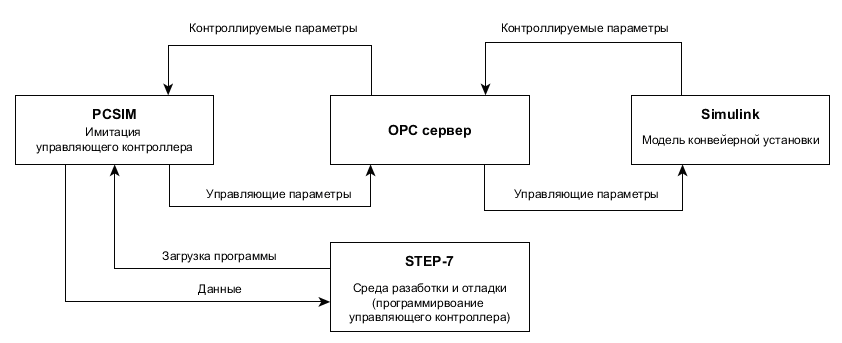
\includegraphics [scale=0.75] {imitation.png}
  \caption{Общая схема взаимодействия компонентов имитационной среды}
  \label{img.5.imitation}  
\end{figure}

В реальных системах управления значения требуемых технологических параметров объекта получают с помощью измерительных устройств (датчиков), значения этих параметров передаются в управляющий контроллер, где производятся необходимые вычисления на основе алгоритмов управления технологическим процессом и формируются сигналы управления, передаваемые на исполнительные устройства объекта. В имитационной среде значения требуемых технологических параметров получают от модели технологического процесса. Эти значения передаются в среду моделирования работы управляющего контроллера. Другими словами, среда моделирования работы управляющего контроллера и среда Simulink, в которой реализована исследуемая модель конвейера, являются независимыми компонентами, поэтому очень важным аспектом является обеспечение передачи данных в реальном времени -- только в этом случае можно говорить о корректности имитации реального технологического процесса. 

Для передачи данных между компонентами имитационной среды был использован OPC-сервер -- программное обеспечение, соответствующее стандарту OPC и предназначенное для совместной работы средств автоматизации. Стандарт ОРС описывает универсальный фиксированный интерфейс обмена данными с любыми устройствами и программным обеспечением []. Программное обеспечение, соответствующее стандарту ОРС, может быть использовано не только для взаимодействия SCADA-систем с аппаратным обеспечением систем управления, но и для обмена данными между любыми источниками и потребителями данных. Эта возможность была использована при разработке и отладке комплексной системы управления конвейером.
 
Возможность получения корректных результатов при разработке и отладке системы управления и ее компонентов в имитационной среде, применимых в реальных условиях эксплуатации, обеспечивается выполнением следующих условий:
\begin{itemize}
\item использованием математической модели объекта управления, описывающей его с достаточной точностью;
\item использованием средств взаимодействия компонентов, обеспечивающих передачу данных в реальном времени;
\item использованием специального имитационного программного обеспечения, совместимого с выбранным оборудованием.
\end{itemize}

Взаимодействие между моделью конвейера и управляющей программой в среде моделирования работы управляющего контроллера осуществляется следующим образом. Simulink обеспечивает передачу требуемых сигналов в реальном времени OPC-сервер посредством блока \textit{OPC Write} из набора компонентов \textit{OPC Toolbox}. C OPC-сервера эти величины считываются программой в имитационной среде, после чего программа производит вычислительные операции, формирующие сигналы управляющих воздействий. Эти сигналы передаются в реальном времени на OPC-сервер, с которого они считывается Simulink посредством блока \textit{OPC Read} из набора компонентов \textit{OPC Toolbox}.

\section{Выводы по главе \ref{chapt5}} \label{sect5_5}

В настоящей главе описана структура и предложен вариант реализации комплексной автоматической системы управления конвейерной установкой, реализующей алгоритмы управления, использование которых позволяет повысить эффективность работы конвейера, увеличить срок службы конвейерной ленты -- наиболее дорогостоящего компонента конвейерной установки. Одним из компонентов системы является реализация разработанного в главе \ref{chapt4} алгоритма предварительного управляемого торможения конвейера. 

Описанный вариант реализации системы управления включает в себя предложения по выбору аппаратного обеспечения (программируемых контроллеров, коммуникационных модулей, источников питания), размещению первичных преобразователей для получения информации от объекта управления, а также описывает решение задачи распределенного сбора данных и управления перемещающимися компонентами конвейерной установки. В главе также представлены результаты разработки программного обеспечения, реализующего алгоритмы управления системы на промышленном языке программирования стандарта МЭК 61131-3. Исходные коды программ реализации алгоритмов возможно использовать на любом промышленном вычислительном оборудовании, поддерживающем этот стандарт. Это исключает жесткую привязку разработанного программного обеспечения к выбранному оборудованию и позволяет при необходимости построить систему управления с использованием другого аппаратного обеспечения или использовать  разработанное программное обеспечение при построении других автоматических систем управления.